% !TeX encoding   = UTF-8
\documentclass[12pt]{article}

\usepackage{sbc-template}

\usepackage{graphicx,url}
\usepackage[brazil]{babel}
\usepackage[utf8]{inputenc}
\usepackage{graphicx}   %Package para figuras
\usepackage{enumerate}
\usepackage{tabularx}
\usepackage{multirow}
\usepackage[table,xcdraw]{xcolor}


\sloppy

\title{Ferramentas para Business Report \\
com Suporte à Linguagem XBRL - \\
Revisão Sistemática da Literatura}

%\author{Vagner Clementino\inst{1}}

\address{Departamento de Ciência da Computação\\
        Universidade Federal de Minas Gerais (UFMG)\\
%  \email{vagnercs@dcc.ufmg.br}
}

\date{Dezembro de 2015}
\begin{document}

\maketitle

%\begin{abstract}
%  This meta-paper describes the style to be used in articles and short papers
%  for SBC conferences. For papers in English, you should add just an abstract
%  while for the papers in Portuguese, we also ask for an abstract in
%  Portuguese (``resumo''). In both cases, abstracts should not have more than
%  10 lines and must be in the first page of the paper.
%\end{abstract}

\begin{resumo}
 A XBRL (\textit{eXtensible Business Report Language})
é uma linguagem para divulgação e intercâmbio de informações financeiras
baseada em XML. Devido a sua crescente adoção no mundo, especialmente pelas
entidades públicas, existe a necessidade da aquisição ou desenvolvimento de
ferramentas que deem suporte à XBRL. Visando ajudar nesta tomada de decisão foi
realizada uma Revisão Sistemática da Literatura com objetivo de levantar as
ferramentas para Business Report que dão suporte à XBRL.
\end{resumo}


\section{Introdução}
\label{sec:contexto}

Uma \textit{Revisão Sistemática da Literatura} - SLR (do inglês Systematic Literature Review) é uma
metodologia científica cujo objetivo é identificar, avaliar e interpretar
\textit{toda} pesquisa \textit{relevante} sobre uma questão de
pesquisa, área ou fenômeno de
interesse\cite{keele2007guidelines,wohlin2012experimentation}. Por se tratar de uma metodologia científica deve estar amparada por um processo conciso para a sua correta execução. Neste sentido, trabalhos que descrevem boas práticas na condução de uma SLR salientam a necessidade da definição de um protocolo durante a fase de planejamento de uma Revisão \cite{keele2007guidelines, biolchini2005systematic}.

Neste contexto, o presente documento tem por objetivo propor uma Revisão
Sistemática da literatura sobre o tema \textit{ferramentas para Business Report com suporte à linguagem XBRL}. \textit{Relatórios  de Negócio (Business Report)} é o produto final do  processo de divulgação pública de dados operacionais e financeiras de uma organização ou ainda a prestação regular de informações para os gestores dentro de uma empresa visado apoiá-los no processo de tomada de decisão.
\cite{lymer1999business}. Há uma terceira via da área de  Relatórios de Negócio
está relacionada ao processo de prestação de contas por entes públicos aos
governos nacionais. A XBRL (\textit{eXtensible Business Report Language})
é uma linguagem para divulgação e intercâmbio de informações financeiras
baseada em XML \cite{xbrl_conceitos_aplicacoes}. O padrão vem sendo adotado por diversas instituições e empresas em todo mundo com o suporte de um consórcio global\footnote{\url{www.xbrl.org}} com mais de 650 membros que incentivam a criação de jurisdições locais. Atualmente o consórcio conta com 24 jurisdições, sendo que em países como  Estados Unidos, Grã-Bretanha e Austrália, a XBRL já é a linguagem oficial para entrega
de relatórios à órgãos de governo. A Figura \ref{fig:world_map} exibe os países
que estão aderindo à XBRL. Estes países estão com a coloração mais escura no mapa.

\begin{figure}[htb]
\centering
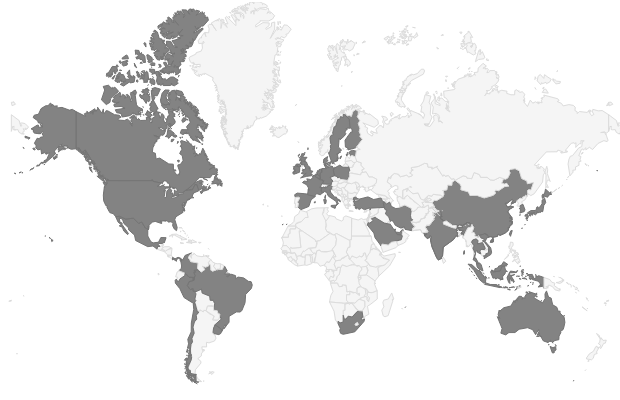
\includegraphics[width=.75\textwidth]{../img/world-map.png}
\caption{O uso da XBRL no mundo}
\label{fig:world_map}
\end{figure}

\section{Justificativa}
\label{sec:problema}

Tendo em vista determinação da Secretaria do Tesouro Nacional, órgão
vinculado ao  Ministério da Fazenda do Brasil, que definiu o XBRL como
padrão para o envio de relatórios de prestação de contas pelos entes
federativos (estados e municípios) por meio do SICONFI – Sistema de Informações Contábeis e Fiscais do Setor Público Brasileiro \cite{nt_03_2013}, surge a necessidade por parte
daquelas organizações do \textit{desenvolvimento ou aquisição} de sistemas de
informação capazes de criar, processar e enviar informações no formato
XBRL. Um cenário onde tal necessidade ocorre é no caso de prefeituras de cidades de pequeno e médio porte que necessitam prestar contas
via \textit{XBRL}, contudo, não possuem conhecimento ou tempo necessário para desenvolver alguma ferramenta que suporte a linguagem.

Neste sentido, verifica-se que existe a demanda por parte das organizações, especialmente as entidades públicas, de referências de qualidade sobre o assunto de \textit{XBRL}. Neste contexto, entende-se que uma Revisão Sistemática da Literatura - SLR  que avaliasse as ferramentas para Business Report que dão suporte ao XBRL pode \textit{subsidiar a tomada de decisão} por parte dos gestores públicos sobre a aquisição de tais ferramentas. Além disso, um trabalho neste sentido poderia subsidiar o desenvolvimento de novas ferramentas que venham preencher as eventuais lacunas existentes nos sistemas atuais. Ademais, traz o foco da comunidade científica sobre um assunto que vêm crescendo bastante nos últimos anos, dentre outros motivos, devido à necessidade das organizações públicas ou privadas de serem cada vez mais transparentes.


\section{Metodologia de Pesquisa}
\label{sec:metodologia}

\subsection{Protocolo da Revisão}
\label{subsec:protocolo}

Uma \textit{Revisão Sistemática da Literatura} - SLR (do inglês Systematic Literature Review) é uma
metodologia científica cujo objetivo é identificar, avaliar e interpretar
\textit{toda} pesquisa \textit{relevante} sobre uma questão de pesquisa, área
ou fenômeno de interesse \cite{keele2007guidelines,wohlin2012experimentation}. Neste trabalho
será utilizada as diretrizes proposta \cite{keele2007guidelines} no qual uma
Revisão Sistemática deve seguir os seguintes passos:

\begin{enumerate}
  \item \textbf{Planejamento}
  \begin{enumerate}
    \item \textit{Identificar a necessidade da Revisão}
    \item \textit{Especificar questões de pesquisa}
    \item \textit{Desenvolver o Protocolo da Revisão}
  \end{enumerate}
  \item \textbf{Condução/Execução}
  \begin{enumerate}
    \item \textit{Seleção dos Estudos Primários}
    \item \textit{Análise da qualidade dos Estudos Primários}
     \item \textit{Extração dos Dados}
     \item \textit{Sintetização dos Dados}
   \end{enumerate}
  \item \textbf{Escrita/Publicação}
  \begin{enumerate}
    \item \textit{Redigir documento com os resultados da Revisão}
    \item \textit{Redigir documento com lições aprendidas}
  \end{enumerate}
\end{enumerate}

Conforme exposto, durante o planejamento da revisão deve desenvolvido um
protocolo com as diretrizes que conduzirão a pesquisa. Além disso devem ser
propostas as questões de pesquisa que devem ser respondidas pelo SLR. Para
esta revisão são propostas as seguintes questões de pesquisa:

\begin{itemize}

  \item \textbf{$Q1$}: Quais são as ferramentas para Relatórios de Negócio que
    suportam a XBRL?
  \item \textbf{$Q2$}: Quais são as funcionalidades comuns as ferramentas
    que possibilitem a comparação entre elas?
  \item \textbf{$Q3$}: Existem casos reais de utilização da ferramenta
    (Estudos de Casos, Whitepapers e etc)?
  \item \textbf{$Q4$}: Qual setor da economia (governos, medicina, setor financeiro) a ferramenta possui histórico de utilização?

\end{itemize}
A partir deste conjunto de questões é possível propor as sentenças de busca que
serão utilizadas na busca dos estudos primários e subsidiar o processo de
extração dos dados daqueles estudos.

\subsection{Critérios de Inclusão e Exclusão}
\label{subsec:inclusao-exclusao}

Nesta seção define-se os critérios para a inclusão de determinado estudo
primário na Revisão. Naturalmente para o estudo ser incluído deverá atender as diretrizes propostas bem
como passar pelo crivo da avaliação de qualidade, conforme disposto na Subseção
\ref{subsec:analise-qualidade}. Neste sentido, um trabalho para ser aceito
como estudo primário deve atender aos seguintes critérios de inclusão:

\begin{itemize}

\item Tem ser publicado a partir de 2008.
\item Estar escrito em língua inglesa.
\item Artigos de Conferência, journals e Whitepapers
\item Dissertações ou Teses apenas se a ferramenta proposta tenha sido
  implementada e testada.
\end{itemize}


No de caso algum estudo recuperado atender qualquer um dos dos seguintes
critérios de exclusão ele deverá ser removido do Revisão mesmo que ele atenda a
algum outro critério de inclusão descritos acima. Os critérios de exclusão
deste trabalho são os seguintes:

\begin{itemize}
\item Trabalhos escritos em outra língua que não a inglesa
\item Documentos duplicados.
\item Livros
\item Dissertações ou Teses apenas se a ferramenta que não há a implementação da
  ferramenta.
\item Literaturas escritas antes do ano de 2008
\end{itemize}

\subsection{Seleção dos Estudos Primários}
\label{subsec:estudos-primarios}

Estudo Primário, no contexto da evidência, é um estudo empírico que investiga
uma questão de pesquisa específica\cite{keele2007guidelines}. No caso de um SLR são os estudos que
possibilitam responder as questões de pesquisa proposta na Revisão. Os guias de boas práticas na condução de uma Revisão Sistemática, especialmente
os da medicina, pregam a necessidade de uma busca exaustiva em diversos tipos
de bases de dados, sejam elas eletrônicas ou não. Não obstante, devido à
evolução das ferramentas de indexação de trabalhos acadêmicos, uma revisão pode
utilizar apenas base de dados eletrônicas sem perda de generalidade. Neste
trabalho, foram utilizadas as bases de dados constantes da Tabela
\ref{tab:base-dados}. Trata-se de uma lista com pequenas alteração da
proposta por \cite{Brereton2007571} com a inclusão de algumas bases,
especialmente o \textit{Google Scholar} e  \textit{XBRL Consortium}. No caso
\textit{Google Scholar} alguns trabalhos demostraram através de suas pesquisa é
possível encontrar 90\% dos artigos passíveis de serem descobertos em outras
bases de dados \cite{yasin2012quality}. Para a base de dados \textit{XBRL
  Consortium} a justificativa vem do fato que ser este o  site da entidade mantenedora do XBRL.

\begin{table}[ht]
\centering
\resizebox{\textwidth}{5cm} \\ \hline
1           & IEEE Xplore                                 & 3              & 0,74\%      \\ \hline
2           & ScienceDirect                               & 100            & 24,57\%     \\ \hline
3           & Springer Link                               & 6              & 1,47\%      \\ \hline
4           & ACM Digital Library                         & 97             & 23,83\%     \\ \hline
5           & Web of Science                              & 9              & 2,21\%      \\ \hline
6           & CiteSeer                                    & 45             & 11,06\%     \\ \hline
7           & Wiley Online Library                        & 54             & 13,27\%     \\ \hline
8           & Scopus Elsevier                             & 8              & 1,97\%      \\ \hline
9           & EL Compendex                                & 9              & 2,21\%      \\ \hline
10          & Google scholar                              & 30             & 7,37\%      \\ \hline
11          & XBRL Consortium                             & 46             & 11,30\%     \\ \hline
\multicolumn{2}{|c|}{Total}                               & 407            & 100,00\%    \\ \hline
\end{tabular}
}
\caption{Base de dados e número de artigos}
\label{tab:base-dados}
\end{table}

Para obter o total de trabalhos exibidos na tabela \ref{tab:base-dados} cada
uma das bases de dados foi consultada com a sentença de busca ``XBRL \textbf{AND} Business Report \textbf{AND} tool
''. Com o objetivo de reduzir o número de documentos recuperados e melhorar a
qualidade dos resultados o seguintes critérios foram aplicados nas ferramentas
de busca: trabalhos publicados a partir de 2008 em que os termos pesquisados
estivessem no título, resumo ou nas palavras-chaves.

Após a primeira consulta realizada conforme descrito anteriormente, uma nova
rodada de consultas era realizada utilizando um \textit{Dicionários de Sinônimos}, que consiste basicamente de um conjunto de
termos similares aos originais que podem aumentar o leque de artigos
recuperados durante a busca. A Tabela \ref{tab:dicionario} exibe o dicionário
de dados que deverá ser utilizado durante a Revisão. A total deste processo foi
obtido um total de \textit{400} trabalhos recuperados.

\begin{table}[ht]
\centering
\resizebox{\textwidth}{!}{%
\begin{tabular}{|c|l|}
\hline
\multicolumn{2}{|c|}{\textbf{DICIONÁRIO DE SINÔNIMOS}} \\ \hline
\textbf{Termo Original} & \multicolumn{1}{c|}{\textbf{Sinônimo}} \\ \hline
XBRL & XML OR XHTML \\ \hline
tool & sofwtare OR  application OR product OR project OR development \\ \hline
Business Report & Finantial Report OR Data Extraction \\ \hline
\end{tabular}
}
\caption{Dicionário de Sinônimos}
\label{tab:dicionario}
\end{table}

\subsection{Decisão de Inclusão e Exclusão}
\label{subsec:decisao-inclusao}

Tendo em vista que os estudo primários foram selecionados de diversas bases de
dados (vide Tabela \ref{tab:base-dados}) ocorreram duplicação de
resultados. Para ajudar na tarefa de remoção de trabalhos duplicados foi utilizado a
ferramenta para a gestão de referências
\textit{JabRef}\footnote{\url{http://jabref.sourceforge.net/}}. Para cada uma
das bases de dados consultadas (Tabela \ref{tab:base-dados}) foi criado um
bando de dados na ferramenta no qual aplicada a funcionalidade de remoção de
duplicada. Trata-se de um processo automatizada cujo os detalhes fogem do
escopo deste texto. Todavia, para os casos em que o \textit{JabRef} não
consegui determinar se dois documentos são duplicados, a ferramenta solicita a
supervisão do usuário. Posteriormente todos os onze bancos de dados criados no
passo anterior foram mesclados em um único para o qual foi solicitada a remoção
de duplicatas. Aproveitando que a ferramenta \textit{JabRef} identifica o tipo
de publicação do trabalho foram removidos os estudo identificados como livros.
Desta forma, ao final este processo o número de \textit{382} trabalhos.

Embora o título de um estudo nem sempre são descritivos o suficiente para
indicar o assunto de estudo, foi adotado o processo de remover os estudos
primários avaliando inicialmente o seu título. Ao final deste processo de
filtro foram \textit{excluídos 202 artigos}. Na terceira etapa, o resumo
(abstract) dos estudos foram utilizados como critérios de escolha. Esta é
última etapa antes da avaliação de qualidade dos estudos (Subseção
\ref{subsec:analise-qualidade}). Apesar da literatura ponderar a necessidade
deste processo de escolha ser realizado aos pares, este procedimento não foi
adotado tendo em vista a impossibilidade de outro pesquisador ou especialista
com a possibilidade de realizar tal tarefa. Ao final deste quatros passos
restaram um total de para serem avaliados segundo os critérios de qualidade
dispostos na Subseção \ref{subsec:analise-qualidade}.

\subsection{Análise de Qualidade}
\label{subsec:analise-qualidade}
Não há como desvincular a qualidade de uma SLR da qualidade dos estudos que a
compõe. Neste sentindo se faz necessário a definição de regras claras de
qualidade a fim de removermos trabalhos que possam causar ameaças aos
resultados da Revisão Sistemática. Para esta Revisão foram utilizados os
seguintes critérios de avaliação da qualidade:

\begin{itemize}
\item Existe uma clara definição do estudo?
\item Existe avaliação da ferramenta proposta bem como discussão dos resultados?
\item O estudo é capaz de responder de forma clara pelo menos 50\% das questões
  de pesquisa?
\end{itemize}

Cada um dos trabalhos escolhidos na etapa de seleção anterior foram validados
no crivo de qualidade proposto. Nesta etapa outros 30
trabalhos foram o excluídos e apenas 29 estudos são permaneceram
para serem utilizados no processo de extração e sintetização dos dados. Na
realidade alguns artigos foram aprovados após a leitura do seu resumo, contudo,
não foi possível acesso ao texto completo dos mesmo que só permitiam acesso
após a compra do mesmo. Findada
a fase de seleção dos estudos podemos visualizar na  Figura \ref{fig:fases}
o número de trabalhos existentes em cada fase de seleção da Revisão.

\begin{figure}[htb]
\centering
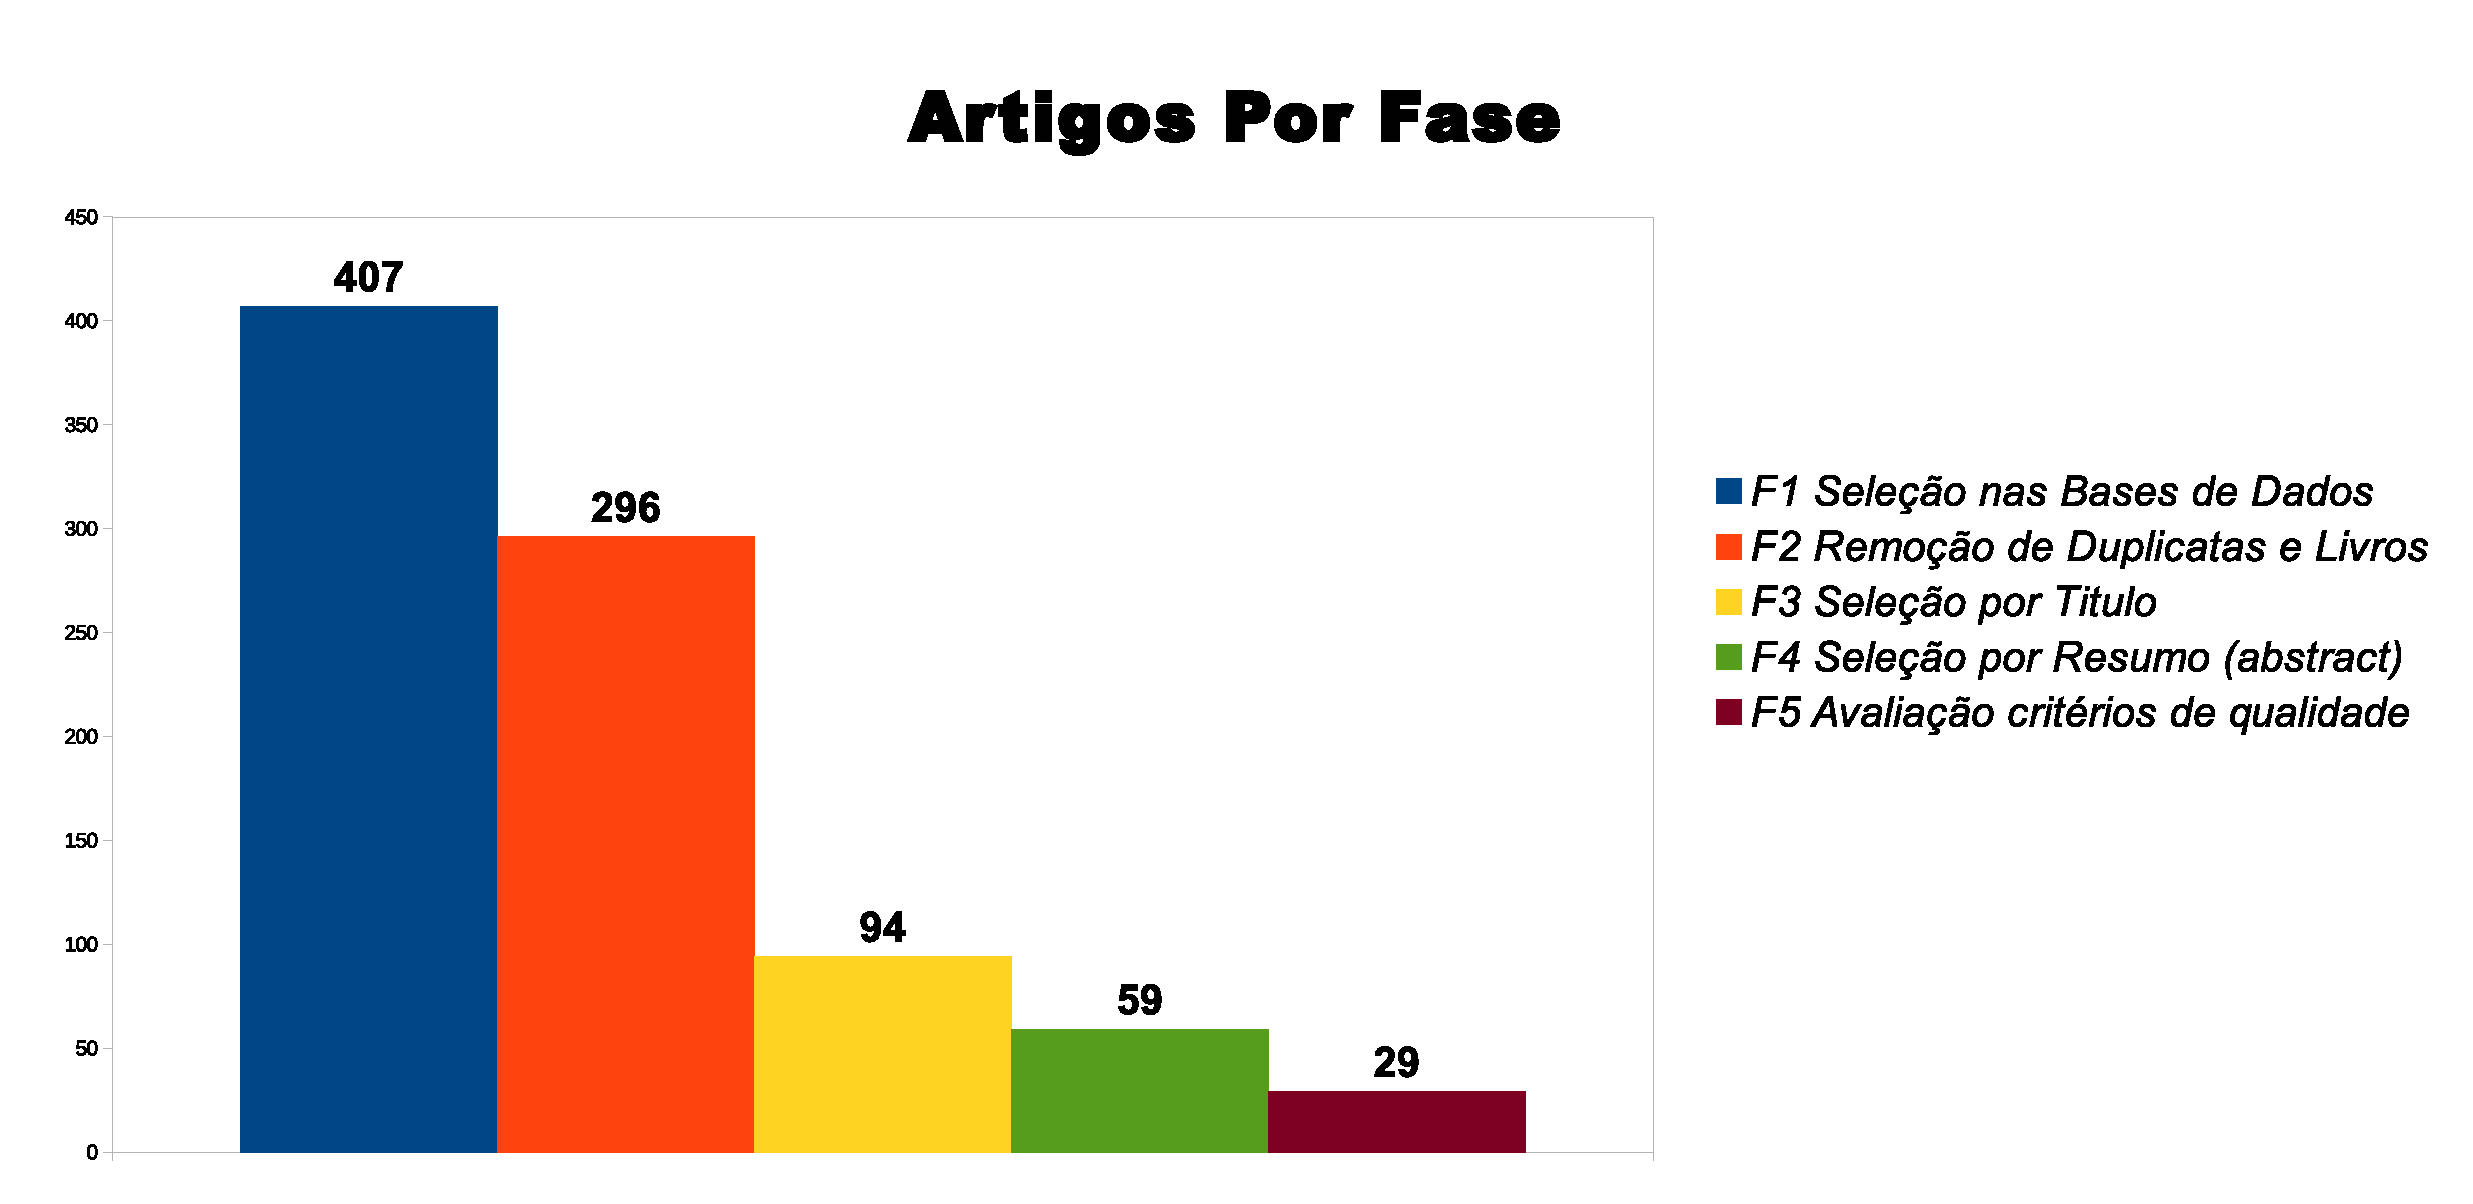
\includegraphics[width=.75\textwidth]{../img/graph_fases.eps}
\caption{Total de artigos em cada fase da SLR}
\label{fig:fases}
\end{figure}


\subsection{Extração dos Dados}
\label{subsec:extracao}

Do total de 29 estudos que foram aprovados pelo processo de
avaliação da qualidade coletou-se dados com base no formulário cujos campos
estão exibidos na Tabela \ref{tab:campos-form}. A extração de dados do estudos
mediante um formulário possibilita o armazenamento das informações para fins de
processamento posterior bem como identificar como cada estudo responde a
determinada questão de pesquisa. Como alguns campos do formulário tem caráter
subjetivo, o campo ``Objetivo do Estudo'' por exemplo, o ideal que as respostas
de cada formulário fosse validade em pares. Todavia, por não haver profissional
para tal atividade este tipo de revisão não foi executada.


\begin{table}[ht]
\resizebox{\textwidth}{!}{%
\begin{tabular}{|c|l|l|}
\hline
\textbf{\#} & \multicolumn{1}{c|}{\textbf{Atributo}} & \multicolumn{1}{c|}{\textbf{Descrição}}                                                      \\ \hline
01          & Identificador do Estudo                & ID único para cada estudo, por exemplo IE01                                                  \\ \hline
02          & Data de Extração                       & Data no qual a extração foi conduzida (DD/MM/YYYY)                                           \\ \hline
03          & Nome do Extrator                       & Nome da pessoa responsável pela extração                                                     \\ \hline
04          & Autor                                  & Autor do estudo                                                                              \\ \hline
05          & Ano                                    & Ano de publicação do estudo                                                                  \\ \hline
06          & Título                                 & Título do Estudo                                                                             \\ \hline
07          & Tipo de Publicação                     & Artigo de journal ou conferência, dissertação, tese ou whitepaper                            \\ \hline
08          & Objetivo do Estudo                     & Quais foram os objetivos do estudo?                                                          \\ \hline
09          & Metodologia do Estudo                  & Quais foram as metodologias utilizadas no estudo?                                            \\ \hline
10          & Descobertas e Resultados               & Quais foram os resultados e descobertas do estudo                                            \\ \hline
11          & Nome da Ferramenta                     & Nome da ferramenta                                                                           \\ \hline
12          & Desenvolvedor                          & Pessoa ou empresa responsável pelo desenvolvimento                                           \\ \hline
13          & URL                                    & Site da internet da ferramenta                                                               \\ \hline
14          & Objetivo da Ferramenta                 & Qual funcionalidade principal da ferramenta                                                  \\ \hline
15          & Tipo de Arquitetura da Ferramenta      & Cliente/Servidor ou Web ou desktop                                                           \\ \hline
16          & Tipo de Licença da Ferramenta          & Software livre ou proprietário                                                               \\ \hline
17          & Avaliação da Ferramenta                & Como a ferramenta foi avaliada                                                               \\ \hline
18          & Estudo de Casos                        & Existe algum estudo de caso ou aplicação real da ferramenta                                  \\ \hline
19          & Ramo de Atuação                          & Qual setor da economia (governos, medicina, setor financeiro) a ferramenta já foi utilizada? \\ \hline
\end{tabular}
}
\caption{Campos do formulário de extração de dados}
\label{tab:campos-form}
\end{table}



\subsection{Sintetização dos Dados}
\label{subsec:sintetizacao}
Nesta etapa do processo foi realizada a coleta, combinação e sintetização dos
dados extraídos de cada estudo  para as etapas finais da revisão sistemática da
literatura. Neste momento o foco é na classificação e sumarização das
informações com o objetivo de responder as questões de pesquisa. Foi utilizado
técnicas de \textit{Estatística Descritiva} \cite{wohlin2012experimentation}
com o objetivo de descrever e apresentar graficamente aspectos interessante do dataset coletado.
\section{Resultados}
\label{subsec:resultados}
Nesta seção discute-se os resultados desta Revisão Sistema tomando como base
cada cada uma das questões de pesquisa propostas. A partir dos 29 estudos que
chegaram à última etapa da Revisão foi possível responder algumas das questões
de pesquisa forma completa e outras de maneira parcial.

A primeira questão proposta foi \textit{$Q1$: Quais são as ferramentas para
  Relatórios de Negócio que suportam a XBRL?}. Esta questão teve como premissa
que possivelmente existiria um pequeno número ferramentas que dariam suporte à
XBRL. Esta expectativa se confirmou conforme pode ser observado pela Tabela \ref{tab:ferramentas}
. Ao final desta SLR consegui-se mapear um total de 29 ferramentas com suporte à
XBRL. Conforme pode ser observado na Tabela \ref{tab:ferramentas} a grande
parte dos sistemas catalogados (26) são proprietários. Apenas um deles é
declarado como software livre (\textit{Arele}) e outros dois são propostos por
artigos de conferência e não há menção quando ao tipo de licença do
trabalho. No tocante à arquitetura a que foi predominante foi
\textit{Cliente/Servidor} correspondendo a um total de 09 ferramentas, seguido
pelos \textit{Framework} com um total de 05 ferramentas.


\begin{table}[htb]
\resizebox{\textwidth}{!}{%
\begin{tabular}{|l|l|l|l|}
\hline
\multicolumn{1}{|c|}{\textbf{Nome da Ferramenta}} & \multicolumn{1}{c|}{\textbf{Desenvolvedor}} & \multicolumn{1}{c|}{\textbf{Arquitetura}} & \multicolumn{1}{c|}{\textbf{Licença}} \\ \hline
Abax XBRL                                         & 2H Software                                 & Framework                                 & Paga                                  \\ \hline
ADDACTIS Pillar3                                  & ADDACTIS                                    & Cliente/Servidor                          & Pago                                  \\ \hline
AGUILONIUS FactsConverter                         & Aguilonius                                  & Plugin Excel                              & Pago                                  \\ \hline
AGUILONIUS XBRL FACTORY SE                        & Aguilonius                                  & Cliente/Servidor                          & Paga                                  \\ \hline
AMANA SmartNotes                                  & AMANA SmartNotes                            & Desktop                                   & Paga                                  \\ \hline
Arele                                             & XBRL community                              & Framework                                 & Código Aberto                         \\ \hline
Batavia XBRL                                      & Batavia XBRL BV                             & Framework                                 & Paga.                                 \\ \hline
Calcbench                                         & Calcbench                                   & Web application                           & Paga                                  \\ \hline
DataTracks                                        & DataTracks                                  & Cliente/Servidor                          & Paga                                  \\ \hline
FinDynamics                                       & FinDynamics                                 & Excel Plugin                              & Paga                                  \\ \hline
FUJITSU Software Interstage XWand                 & Fujitsu                                     & Framework                                 & Paga                                  \\ \hline
Invoke e-Filing for Banks                         & Invoke                                      & Web Application                           & Paga                                  \\ \hline
IRIS Carbon                                       & IRIS Business Services Limited              & Cloud                                     & Paga                                  \\ \hline
Litix                                             & BR-AG                                       & Mobile                                    & Paga                                  \\ \hline
Oracle Hyperion Disclosure Management             & ORACLE                                      & Cliente/Servidor                          & Paga                                  \\ \hline
ParsePort XBRL Converter                          & ParsePort                                   & Web application                           & Paga                                  \\ \hline
ParsePort                                         & AltaNova                                    & Cliente/Servidor                          & Paga                                  \\ \hline
RegulatorWorks                                    & XBRLWorks                                   & Cliente/Servidor                          & Paga                                  \\ \hline
Reporting Standard XBRL                           & Reporting Standard                          & Desktop                                   & Paga                                  \\ \hline
Seahorse                                          & CoreFiling                                  & Cliente/Servidor                          & Paga                                  \\ \hline
Wdesk                                             & Workiva                                     & Web Application                           & Paga                                  \\ \hline
XBRL Processing Engine (XPE)                      & UBPartner                                   & Framework                                 & Paga                                  \\ \hline
xbrlOne Data Editor                               & Semansys Technologies                       & Desktop                                   & Paga                                  \\ \hline
XKUBED                                            & IPHIX                                       & Cliente/Servidor                          & Paga                                  \\ \hline
Yeti                                              & CoreFiling                                  & Web application                           & Paga                                  \\ \hline
XBRL Database Cluster                             & Argyris Argyrou , Andriy Andreev            & Cliente/Servidor                          & N/A                                   \\ \hline
XBRL Audit Assistant                              & Efrim Boritz \& Won Gyun No                 & Desktop                                   & N/A                                   \\ \hline
\end{tabular}
}
\caption{Ferramentas com Suporte à XBRL}
\label{tab:ferramentas}
\end{table}

A segunda questão foi \textit{$Q2$: Quais são as funcionalidades comuns as ferramentas
    que possibilitem a comparação entre elas?} no qual gostaria de se verificar
  quais as funcionalidades são mais frequentes nas ferramentas possibilitam
  desta forma verificar quais atividades relativas à XBRL estão implementadas
  nas ferramentas. O fato de conhecer as funcionalidades permite a definição de
  critérios de seleção entre as ferramentas. A figura \ref{fig:funcionalidades}
  a frequência de ocorrência de algumas funcionalidades nas ferramentas
  recuperadas. É possível verificar que as funcionalidades de \textit{criação,
    validação e visualização} de Documentos de Instância são as mais frequentes
  entres os sistemas. Um documento de instância é uma coleção de fatos que
  juntos formam um relatório financeiro. Tecnicamente, um documento de
  instância é um documento XML com um elemento raiz \textit{xbrli:xbrl}
  \cite{xbrl_conceitos_aplicacoes}. Na prática um documento de instância é
  fonte de dados para a geração de relatórios em XBRL. Outro fato interessante
  demonstrado na Figura \ref{fig:funcionalidades} é que as cinco
  funcionalidades com maior frequência correspondem a mais de 50\% das
  funcionalidades existente nas ferramentas. Este dados pode servir como base
  para o desenvolvimento de um novo sistema de suporte à XBRL tomando estas
  funcionalidades como base.


\begin{figure}[htb]
\centering
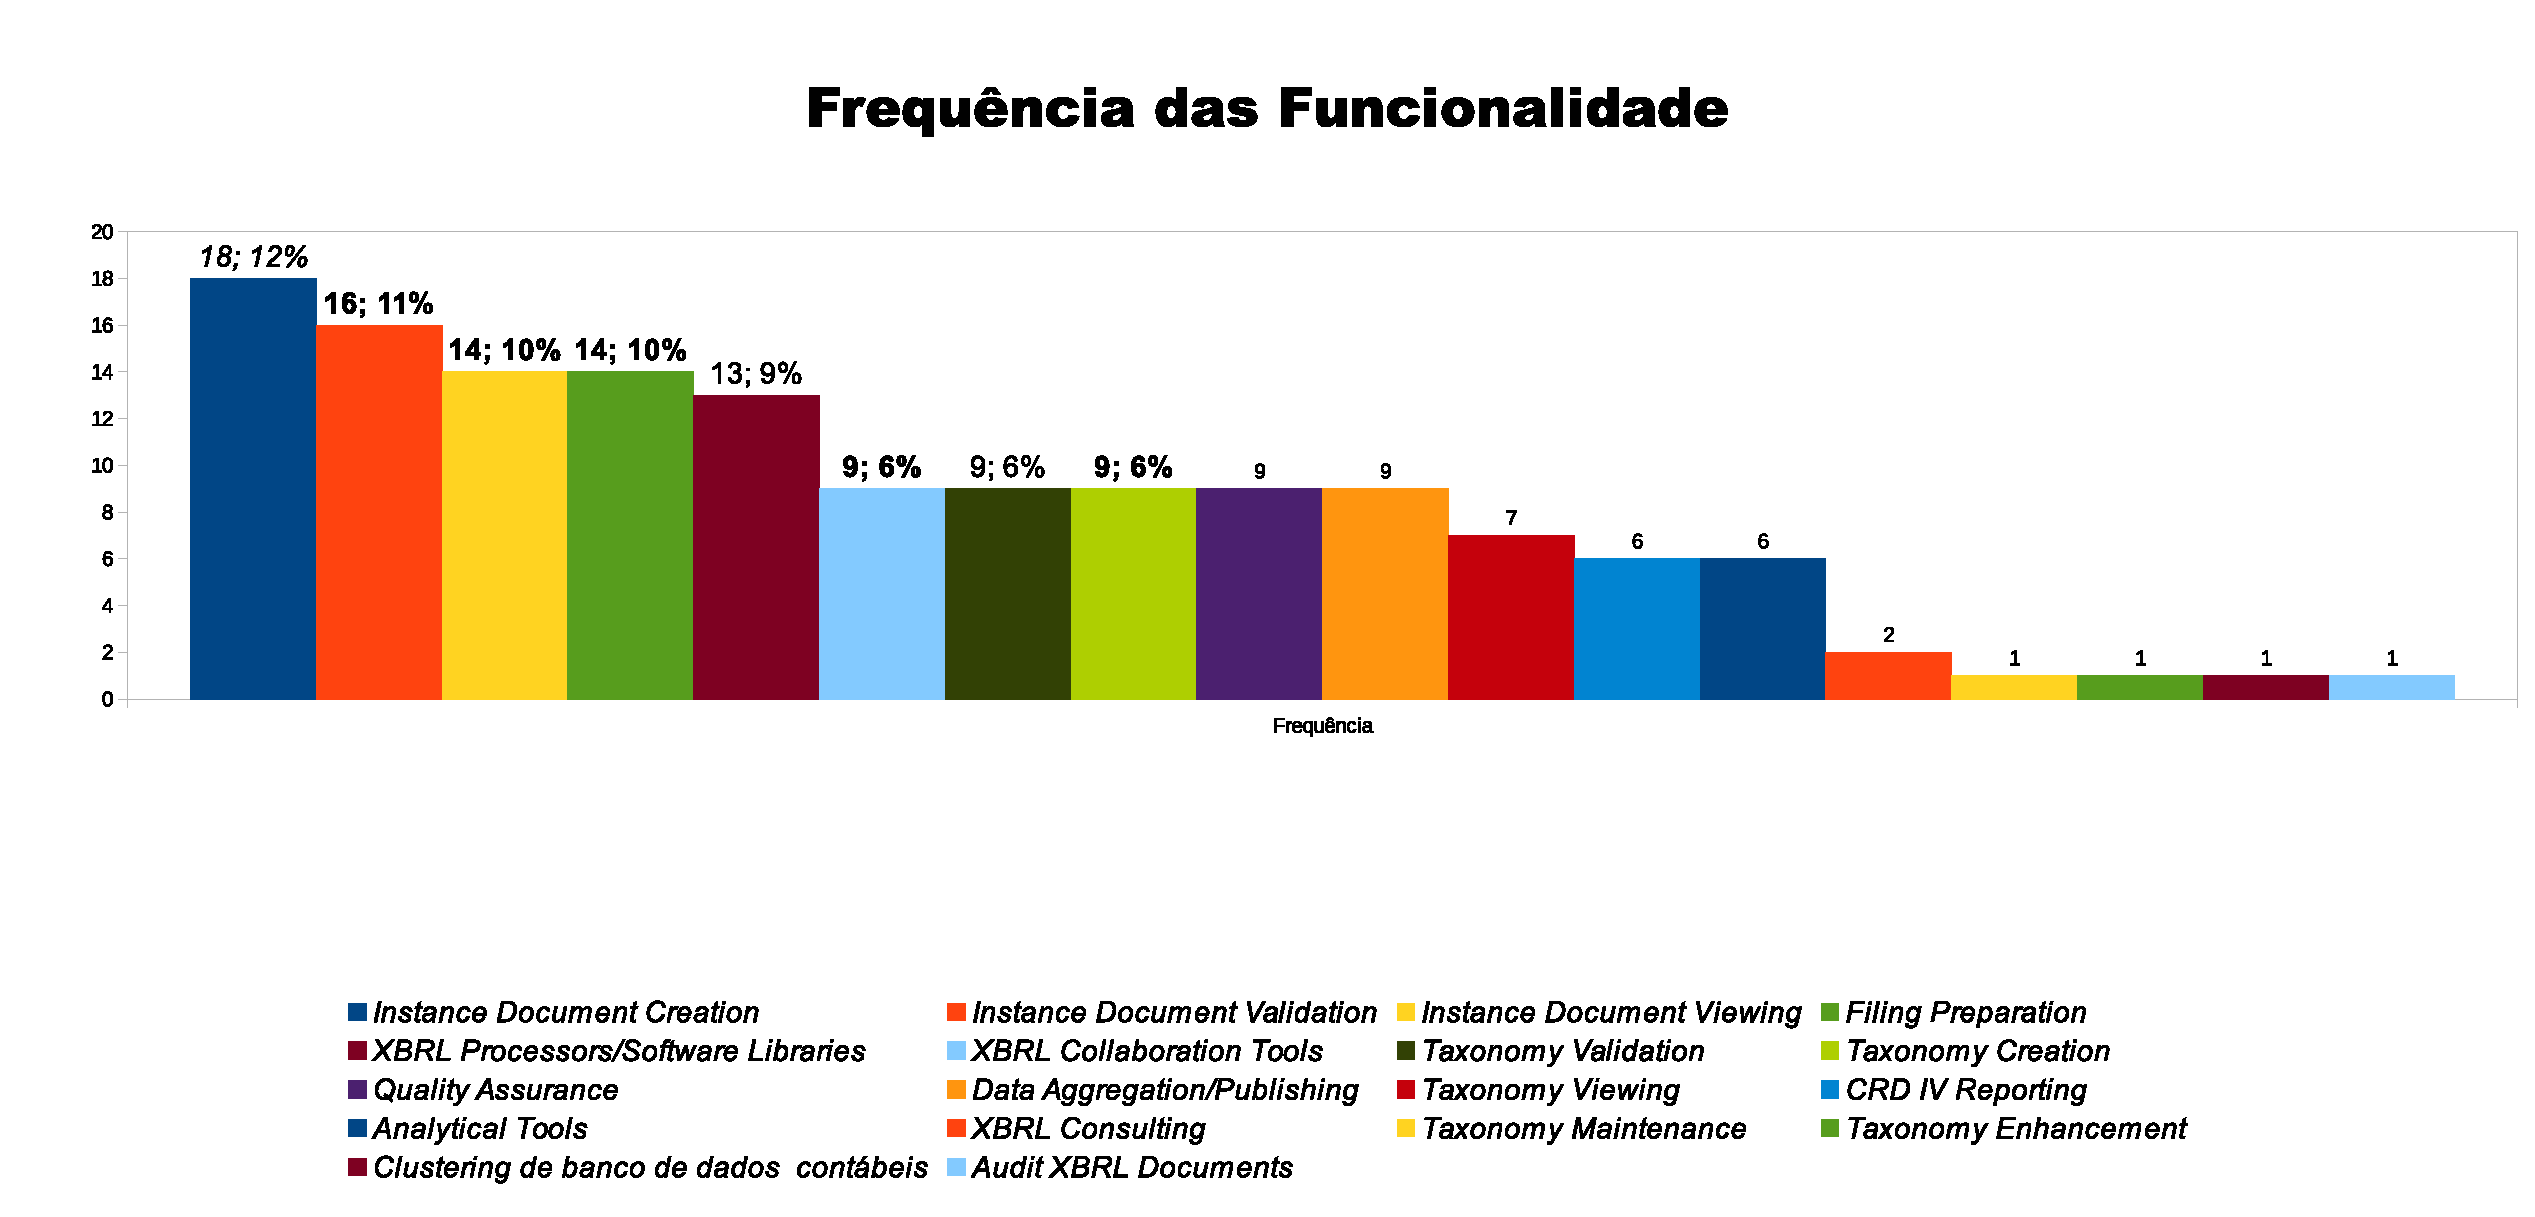
\includegraphics[width=\textwidth]{../img/graph_funcionalidades.eps}
\caption{Frequência das funcionalidades das ferramentas}
\label{fig:funcionalidades}
\end{figure}

A terceira questão de pesuqisa \textit{$Q3$: Existem casos reais de utilização da ferramenta
    (Estudos de Casos, Whitepapers e etc)?} tem como objetivo levantar as
  avaliações práticas das ferramentas propostas. Apesar de grande parte dos
  documentos recuperados se tratarem de \textit{whitepapers} não foi possível
  verificar em nenhum deles a avaliação prática das ferramentas. Há menções de
  clientes  que utilizam a ferramenta e de nichos de mercado no qual o sistema
  está inserido (\textit{$Q4$}. Todavia, não há elementos que possibilitem
  responder \textit{$Q3$}.

A ultima questão proposta neste estudo \textit{$Q4$: Qual setor da economia
  (governos, medicina, setor financeiro) a ferramenta possui histórico de
  utilização?} tem por objetivo verificar a expertise nas ferramentas em
determinados ramos da economia. No caso de alguma organização tomar a decisão
de adquirir um produto ele poderia estar interessada se empresa fornecedora
possui conhecimento das especificidades do setor em que ela está inserida. Do
total de 29 trabalhos que compõe esta Revisão Sistemática apenas em 13 foi
possível definir esta informação. A Figura \ref{fig:setores} exibe os setores
de atuação das ferramentas de modo geral. Conforme esperado bancos e mercado
financeiro são os setores onde as ferramentas mais tem atuado. Um dado que não
era esperado a baixa atuação do setor público (Governo) onde a implantação da
XBRL obedece à fatores legais.

\begin{figure}[htb]
\centering
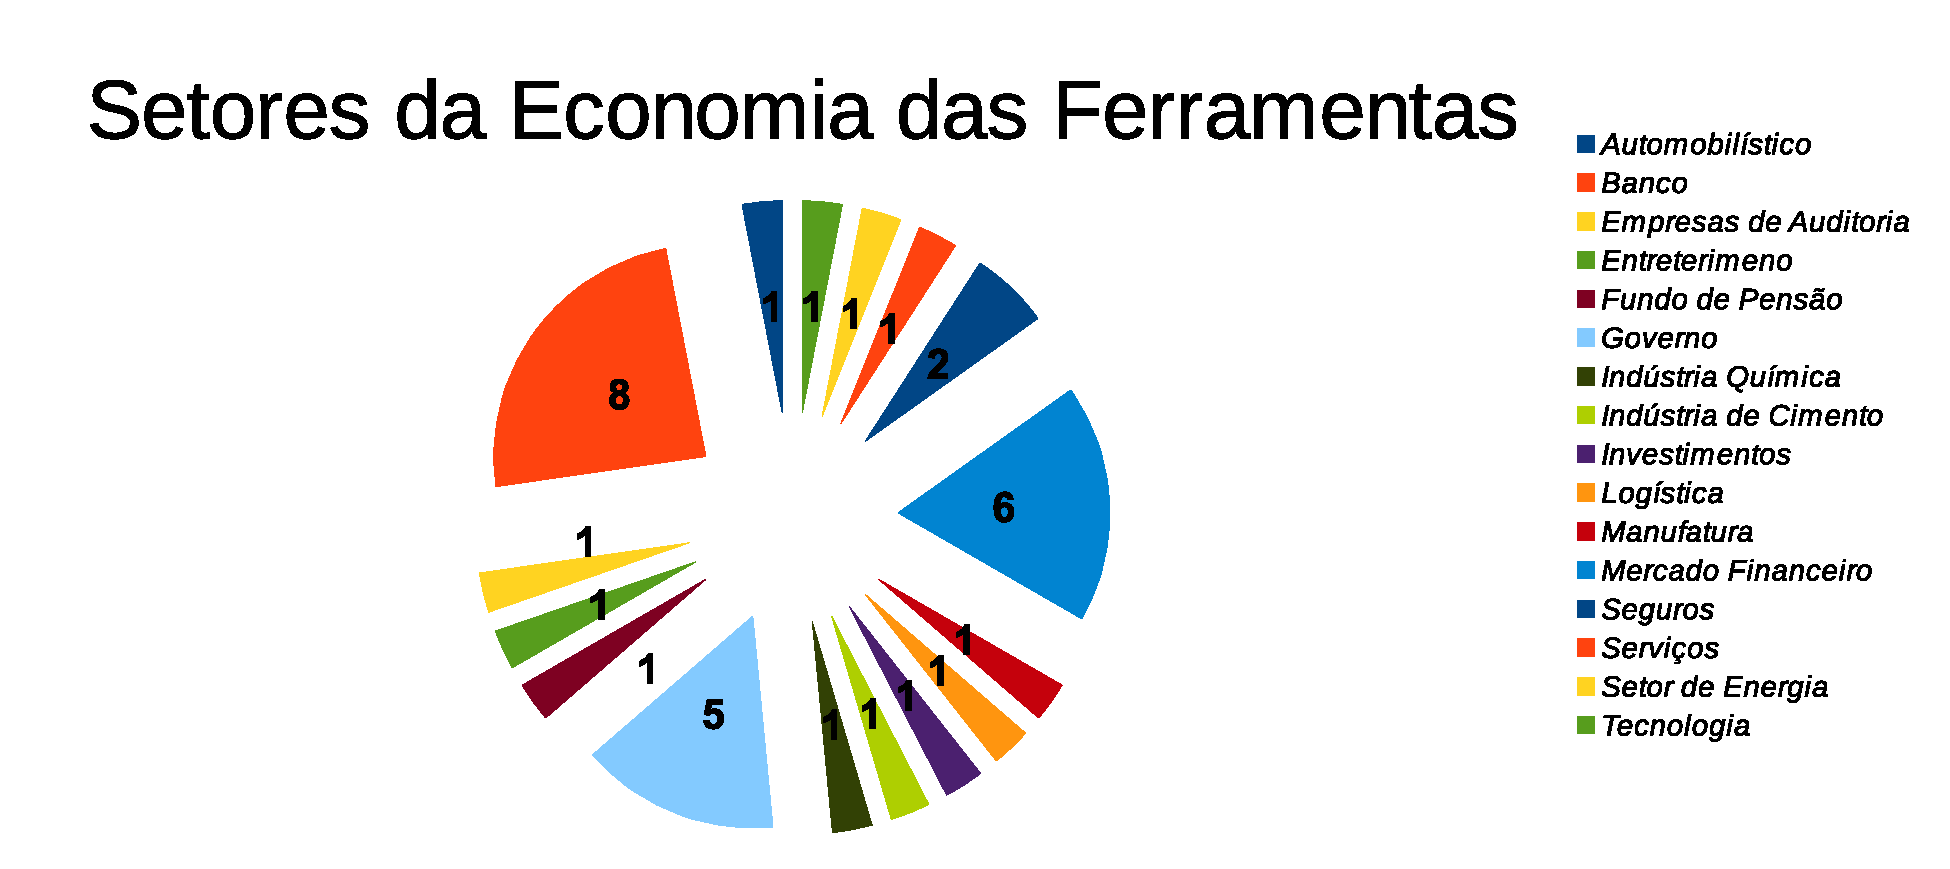
\includegraphics[width=.95\textwidth]{../img/graph_setores.eps}
\caption{Setores de Atuação das Ferramentas}
\label{fig:setores}
\end{figure}

\section{Ameaças à Validade}
\label{sec:ameacas}
Nesta seção discute-se as ameaças aos resultados apresentados neste estudo. Uma
primeira ameaça está relacionada ao fato de ter havido uma validação aos pares
para aceitação dos estudos. O fato de não haver um outro pesquisador para
ponderar quando surgia dúvidas quanto à aceitação de um trabalho pode levar a
algum víes nos resultados do trabalho.

Um segundo fator de ameaça está no fato de que alguns artigos não foram obtidos em sua versão completa porque exigiam a
sua aquisição. Desta forma, nem todo os universo de artigos foi efetivamente
avaliado. Não obstante, o número de estudos nesta situação foi pequeno (03
artigos) sendo portanto uma ameaça de baixo impacto nos resultados.

A última ameaça a validade deste trabalho está relacionado ao tipo de trabalhos
utilizados. A grande parte dos estudos utilizados é do tipo whitepapers que são
classificados como \textit{gray literature}. A utilização deste tipo de
referência têm impacto na qualidade dos resultados. Contudo, devido à
característica deste trabalho este tipo de referência não poderia ser
ignorado.

\section{Conclusão}
\label{sec:conclusao}

Neste trabalho foi realizada uma Revisão Sistemática da Literatura (SLR) seguindo as
diretrizes propostas por \cite{keele2007guidelines} com o objetivo de analisar
as ferramentas que possuem suporte à XBRL. A SLR iniciou com 407 trabalhos e
após a aplicação de critérios de inclusão/exclusão chegou a um total de 29
estudos. A partir destes 29 estudos foi possível responder três das quatros
questões de pesquisa propostas. Os resultados demostram que exitem um número
significado de ferramentas que dão suporte à linguagem XBRL cujas
funcionalidades cobrem os principais requisitos para geração de relatórios em
XBRL, como a criação de objetos de instância por exemplo. Verificou-se ainda
que as ferramentas encontradas têm atuação especialmente nos setores
financeiros e bancários. Existe uma grande possibilidade de crescimento no
setor público.


\bibliographystyle{sbc}
\bibliography{../bib/slr_xbrl_tools}

\end{document}
